\documentclass[
  a4paper,
  upppercaseChapter,
  normalTOC,
  noIndentAnAp,
  fancyPlainHeader,
  samePageChapter
]{academix/academix}

% ------------------------------------------------------------------
% HYPERLINKS AND PDF CONFIGURATION
% ------------------------------------------------------------------

% Enables hyperlinks and defines their appearance
\usepackage[
  bookmarks,
  colorlinks,
  citecolor=black,
  urlcolor=blue,
  linkcolor=black,
  pdfpagemode=UseNone
]{hyperref}

% ------------------------------------------------------------------
% MATHEMATICS SUPPORT
% ------------------------------------------------------------------

% Math support for advanced typesetting (equations, theorems, symbols):
% - amsmath: Advanced math typesetting
% - amsfonts: Extra math fonts
% - amssymb: Additional math symbols
% - amsthm: Theorem-like environments (theorems, lemmas, etc.)
\usepackage{amsmath, amsfonts, amssymb, amsthm}

% Use Times-like font (newtxtext and newtxmath) for both text and math symbols
\usepackage{newtxtext, newtxmath}

% ------------------------------------------------------------------
% FONT AND ENCODING SETTINGS
% ------------------------------------------------------------------

% Set font encoding to T1 for proper handling of special characters (accents, etc.)
\usepackage[T1]{fontenc}

% Set Helvetica as the default sans-serif font (similar to Arial)
% - \sfdefault: Use sans-serif fonts for the entire document
\usepackage{helvet}
\renewcommand{\familydefault}{\sfdefault}

% ------------------------------------------------------------------
% LANGUAGE SUPPORT
% ------------------------------------------------------------------

% Language support for English (proper hyphenation and text rules)
\usepackage[english]{babel}

% ------------------------------------------------------------------
% CITATION MANAGEMENT
% ------------------------------------------------------------------

% APA Style
\usepackage{cite}
\bibliographystyle{apalike}

% Proper formatting and line breaking for URLs
\usepackage{url}

% ------------------------------------------------------------------
% TABLES
% ------------------------------------------------------------------

% Professional-quality tables with enhanced rules and spacing
\usepackage{booktabs}

% Support for large tables that can span multiple pages
% (not compatible with two column)
\usepackage{longtable}

% Combines longtable with tabularx for dynamic column width adjustment in large tables
\usepackage{ltxtable}

% ------------------------------------------------------------------
% FLOATS AND GRAPHICS
% ------------------------------------------------------------------

% Enhanced control over float objects (figures, tables):
% - Allows precise placement of floating objects using the [H] option
\usepackage{float}

% Graphics and images support:
% - pdftex: Use PDFLaTeX engine for image handling
% - graphicspath: Set the directory for images to 'figures/'
% - DeclareGraphicsExtensions: Define preferred image file formats (PDF, JPEG, PNG, JPG)
\usepackage[pdftex]{graphicx}
\graphicspath{{figures/}}
\DeclareGraphicsExtensions{.pdf,.jpeg,.png,.jpg}

% Insert external PDF documents into the LaTeX document
\usepackage{pdfpages}

% ------------------------------------------------------------------
% MISCELLANEOUS
% ------------------------------------------------------------------
\renewcommand{\customChapterMark}[1]{\markboth{#1}{}}
\renewcommand{\customSectionMark}[1]{\markright{#1}{}}
\newcommand{\source}[1]{\\Source: {#1}}

\customAuthor{Adnane El Bouhali, Saba Shahsavari, William Liaw}
\customTitle{Visualizing Olympic Migration and Medal Trends: A Geopolitical Perspective}
\location{Palaiseau}
\customDate{2024}

\advisor{Emmanuel Pietriga}
\minipageText{Report submitted for the Data Visualization course (CSC\_51052) as part of the Master Data AI at Institut Polytechnique de Paris.}

\begin{document}

% -------------
% External part
% -------------
\coverPage


% -------------
% Internal part
% -------------

% Pre-textual elements
\backCover
\pagenumbering{roman}
\begin{abstract}

    This report presents a data visualization project focused on analyzing athlete migration, geopolitical influences, and Olympic medal performance during the Olympic Games from 1986 to 2018. Using a combination of datasets, including Olympic medal counts, population data, and geopolitical events, we explore key trends such as migration patterns of athletes, medals per capita, and temporal medal accumulation across countries. The visualizations are designed to reveal the relationship between global political events and athletic representation, as well as how countries perform in relation to their population size. Interactive visualizations, including flow maps, choropleth maps, and line charts, were implemented using D3.js to offer a comprehensive analysis of the data. The project underscores the value of visualizing complex, multi-dimensional datasets to derive meaningful insights into historical and geopolitical factors affecting Olympic performance.

    \vspace{1\baselineskip}

    \textbf{Keywords:} Olympic Games, athlete migration, geopolitical impact, medals per capita, data visualization, D3.js, temporal trends, choropleth maps, interactive visualizations.

\end{abstract}


\begin{summary}

    Ce rapport présente un projet de visualisation de données axé sur l'analyse des migrations d'athlètes, des influences géopolitiques et de la performance des médailles aux Jeux Olympiques de 1986 à 2018. En utilisant une combinaison de jeux de données, incluant les comptes des médailles olympiques, les données de population et les événements géopolitiques, nous explorons les principales tendances telles que les migrations d'athlètes, le nombre de médailles par habitant et l'accumulation temporelle de médailles par pays. Les visualisations sont conçues pour mettre en lumière les relations entre les événements politiques mondiaux et la représentation athlétique, ainsi que les performances des pays en fonction de leur taille démographique. Des visualisations interactives, incluant des flux migratoires, des cartes choroplèthes et des graphiques linéaires, ont été implémentées à l'aide de D3.js afin d'offrir une analyse complète des données. Ce projet souligne l'importance de la visualisation de jeux de données complexes et multidimensionnels pour extraire des informations significatives sur les facteurs historiques et géopolitiques influençant la performance olympique.



    \vspace{1\baselineskip}

    \textbf{Palavras-chave:} Jeux Olympiques, migration des athlètes, impact géopolitique, médailles par habitant, visualisation de données, D3.js, tendances temporelles, cartes choroplèthes, visualisations interactives.

\end{summary}



\listoffigures
\listoftables
\input{doc/abbreviations}
\begin{listofsymbols}{1000}
	\item [$\Delta(h)$] Assinatura di\' adica
\end{listofsymbols}

\tableofcontents

% Textual elements
\pagenumbering{arabic}
\chapter{Introduction} \label{chap:intro}

The Olympic Games serve as a remarkable global stage where athletes from various countries compete, showcasing their skills while embodying the cultural and historical narratives of their nations. Over more than a century, the Games have generated a rich repository of data that reflects the evolution of athletic participation, medal distributions, and international representation.

This project leverages advanced data visualization techniques to explore trends and patterns in the Olympic Games from 1986 to 2022. The focus is on uncovering insights into athlete migration and medal performance, using datasets sourced primarily from the Kaggle-hosted Olympic Games Medals 1986-2022 repository \cite{olympic_19862022}. Through interactive visualizations created with tools like D3.js \cite{d3}, we aim to provide an intuitive understanding of the relationships and dynamics underpinning Olympic performance over time.

The following sections outline the dataset, the methodologies employed for data preparation and analysis, and the results derived from the visualizations. %This report emphasizes the role of data visualization in interpreting complex datasets and uncovering meaningful historical and competitive trends.


\chapter{Dataset Overview} \label{chap:dataset}

This project relies on the \textit{Olympic Games Medals 1986-2022} dataset, sourced from Kaggle \cite{olympic_19862022}. This dataset was originally scraped from the official International Olympic Committee website \cite{olympics}, ensuring its alignment with authoritative data sources. It consists of multiple files, each providing specific details about athletes, medal outcomes, event results, and hosting nations. Key files include:

\begin{itemize}
    \item \texttt{olympic\_athletes.csv}: Details about athletes, including demographics and participation history.
    \item \texttt{olympic\_medals.csv}: Records of medals awarded across events and disciplines.
    \item \texttt{olympic\_hosts.csv}: Information about hosting cities, countries, and the duration of each Olympic event.
    \item \texttt{olympic\_results.csv}: Comprehensive details on event results, including participants and rankings.
\end{itemize}

Despite its extensive coverage, the raw dataset required significant preprocessing and cleaning to address inconsistencies and prepare it for analysis.

\section{Inconsistent Data Entries}

The raw dataset contained several inconsistencies in data entries that required attention during the preprocessing phase. Two significant issues encountered were duplicate records and invalid birth years. These problems had to be resolved to ensure the dataset's reliability and accuracy for analysis.

\subsection{Duplicate Records}

Duplicate entries for athletes and events were present in the dataset, leading to redundancies and inaccuracies. For instance, multiple records existed for the same athlete across different events or Olympic appearances, making it challenging to analyze unique participation trends. These duplicate entries were systematically identified using key attributes, such as athlete names, event details, and medal information, and subsequently removed to maintain data integrity.

\subsection{Invalid Birth Years}

Another major inconsistency was the presence of invalid or missing birth years for athletes. Implausible values, such as negative birth years or years indicating extreme ages (e.g., over 150 years), were identified in the dataset. These anomalies introduced inaccuracies in calculating athletes' ages at their first Olympic appearance and other related analyses.

To address this, reasonable age boundaries for Olympic participation were established based on historical records. According to sources, the youngest known Olympian was 10 years old \cite{youngest_olympian}, and the oldest recorded Olympian was 73 years old \cite{oldest_olympian}. Using these references, red shaded regions in the visualizations highlight implausible age values falling outside this range.

Figure \ref{fig:birth_years} shows the distribution of athletes' birth years by their first Olympic appearance, with anomalies clearly visible as athletes cannot have their first Olympic appearance before the year their were born. The red shaded region highlights implausible values, including negative ages and values exceeding typical human lifespans. Similarly, Figure \ref{fig:athlete_ages} illustrates the distribution of athletes' ages at their first Olympic appearance.

\begin{figure}[ht]
    \centering
    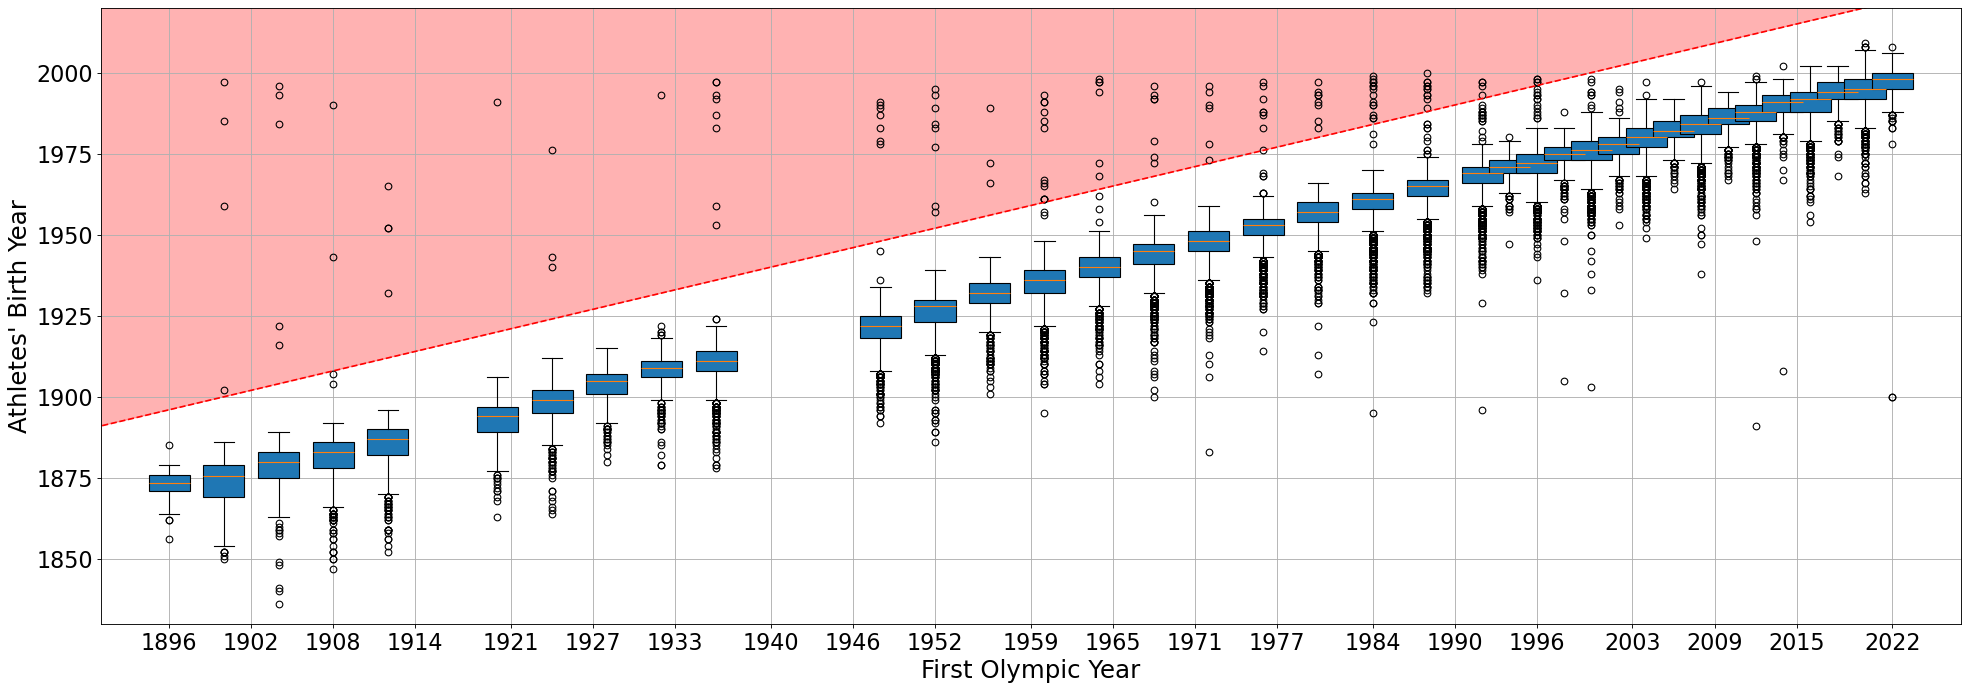
\includegraphics[width=\textwidth, keepaspectratio]{Distribution of Athletes' Birth Years by First Olympic Appearence.png}
    \caption{Distribution of Athletes' Birth Years by First Olympic Appearance}
    \label{fig:birth_years}
\end{figure}

\begin{figure}[ht]
    \centering
    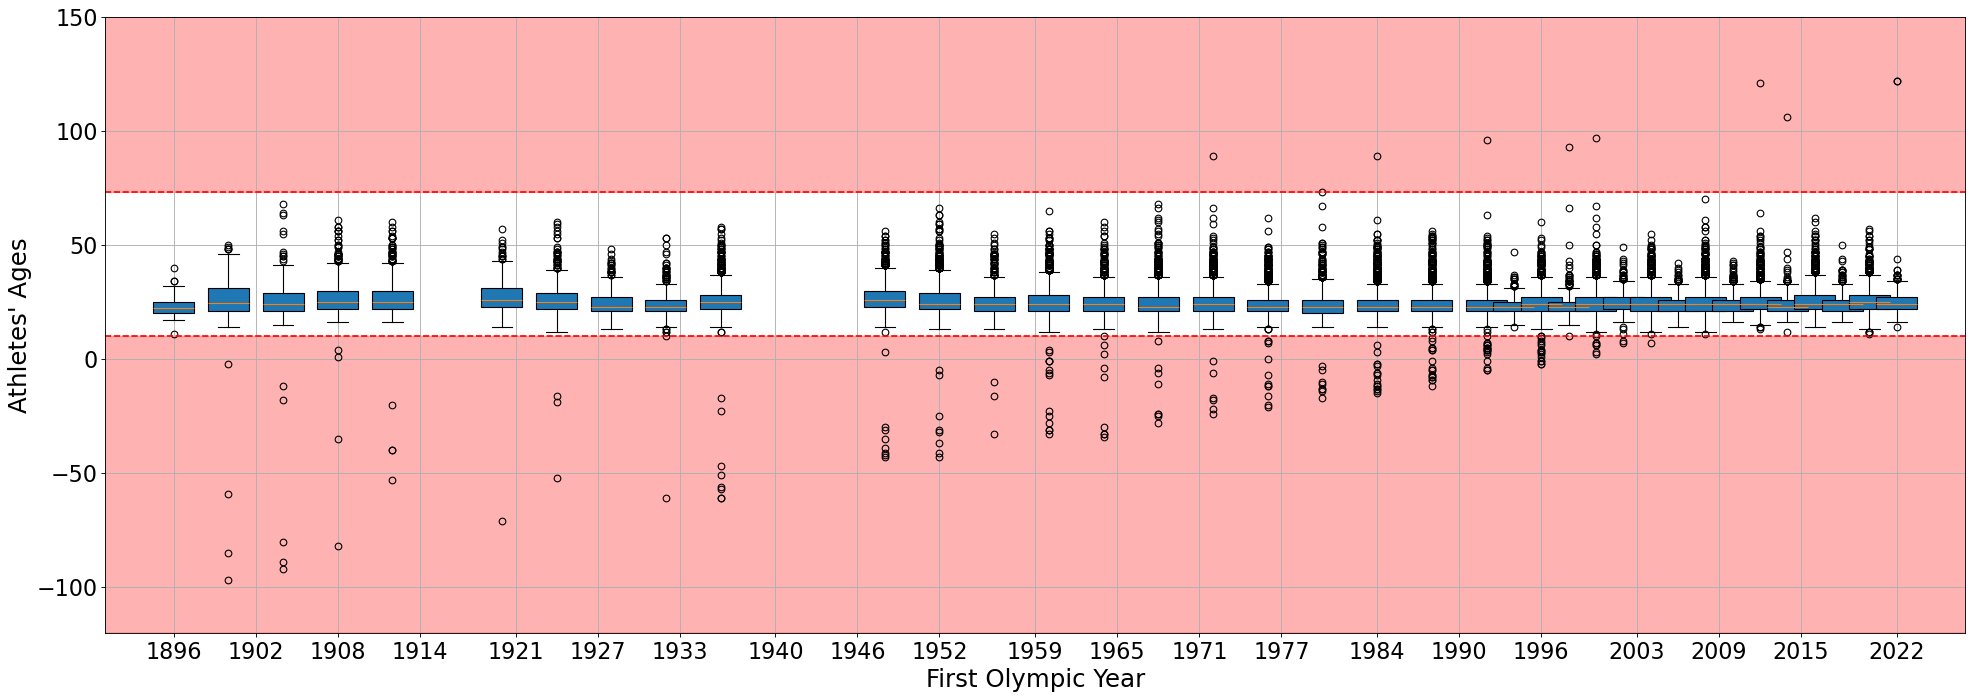
\includegraphics[width=\textwidth, keepaspectratio]{Distribution of Athletes' Ages at Their First Olympic Appearence.png}
    \caption{Distribution of Athletes' Ages at Their First Olympic Appearance}
    \label{fig:athlete_ages}
\end{figure}

\section{Ambiguous Geographical Data}

Geographical data in the raw dataset was often ambiguous or inconsistent. Key issues included:

\begin{itemize}
    \item \textbf{Host City and Country Mapping:} Host cities were inconsistently labeled or lacked corresponding country information. To resolve this, city names were mapped to their respective countries using geocoding tools such as Nominatim \cite{nominatim}.
    \item \textbf{Country Code Discrepancies:} Standardized two-letter (ISO 3166-1 alpha-2) and three-letter (ISO 3166-1 alpha-3) country codes were assigned to all entries to eliminate inconsistencies in naming conventions.
\end{itemize}

By standardizing geographical data, we ensured consistency and improved the dataset's usability for visualizations involving country-specific analyses.


\section{Missing Metadata}

A significant portion of the dataset contained missing or incomplete metadata, particularly for athletes and events. Common issues included:

\begin{itemize}
    \item \textbf{Incomplete Athlete Information:} Some athletes lacked URLs, full names, or demographic details. Such records were filtered out when critical information was unavailable.
    \item \textbf{Unresolved Medalist Metadata:} Certain medalists had incomplete associations with their events or disciplines, which limited their analytical use.
\end{itemize}

These gaps were addressed where possible, and records that could not be resolved were excluded from further analysis.


\chapter{Methodology} \label{chap:method}

The analysis of the Olympic dataset involved a combination of data preprocessing, cleaning, and visualization techniques to uncover meaningful insights. The raw dataset, despite its extensive coverage, required significant preprocessing and cleaning to address inconsistencies and ensure its reliability for analysis. Issues such as duplicate records, missing values, and invalid entries (e.g., unrealistic birth years and medal counts) were identified and carefully resolved. These preprocessing steps laid the foundation for the subsequent analysis, as detailed in the following subsections.

Once the data was cleaned, various visualizations were created to explore patterns and trends in the dataset. Python, with libraries such as \texttt{pandas} and \texttt{matplotlib}, was used to generate preliminary exploratory plots. These static visualizations provided insights into data distributions, temporal trends, and relationships between variables. Examples include boxplots for identifying invalid birth years, line charts for visualizing medal accumulation over time, and scatterplots for exploring correlations.

For more advanced and interactive visualizations, JavaScript and the D3.js library were employed. These tools facilitated the creation of dynamic visualizations, such as choropleth maps for visualizing medal distributions across countries and flow diagrams for illustrating athlete migration patterns. The interactive visualizations incorporated features such as tooltips, zooming, and filtering, allowing users to explore the data in depth and tailor their analysis to specific interests.

This combination of Python for initial exploratory analysis and JavaScript with D3.js for dynamic and interactive visualizations ensured a comprehensive approach to analyzing and presenting the data. Together, these tools provided both high-level summaries and detailed explorations, enhancing the overall analytical process and user experience.

\section{Inconsistent Data Entries}

The raw dataset contained several inconsistencies in data entries that required attention during the preprocessing phase. Two significant issues encountered were duplicate records and invalid birth years. These problems had to be resolved to ensure the dataset's reliability and accuracy for analysis.

\subsection{Duplicate Records}

Duplicate entries for athletes and events were present in the dataset, leading to redundancies and inaccuracies. For instance, multiple records existed for the same athlete across different events or Olympic appearances, making it challenging to analyze unique participation trends. These duplicate entries were systematically identified using key attributes, such as athlete names, event details, and medal information, and subsequently removed to maintain data integrity.

\subsection{Invalid Birth Years}

Another major inconsistency was the presence of invalid or missing birth years for athletes. Implausible values, such as negative birth years or years indicating extreme ages (e.g., over 150 years), were identified in the dataset. These anomalies introduced inaccuracies in calculating athletes' ages at their first Olympic appearance and other related analyses.

To address this, reasonable age boundaries for Olympic participation were established based on historical records. According to sources, the youngest known Olympian was 10 years old \cite{youngest_olympian}, and the oldest recorded Olympian was 73 years old \cite{oldest_olympian}. Using these references, red shaded regions in the visualizations highlight implausible age values falling outside this range.

Figure \ref{fig:birth_years} shows the distribution of athletes' birth years by their first Olympic appearance, with anomalies clearly visible as athletes cannot have their first Olympic appearance before the year their were born. The red shaded region highlights implausible values, including negative ages and values exceeding typical human lifespans. Similarly, Figure \ref{fig:athlete_ages} illustrates the distribution of athletes' ages at their first Olympic appearance.

\begin{figure}[ht]
    \centering
    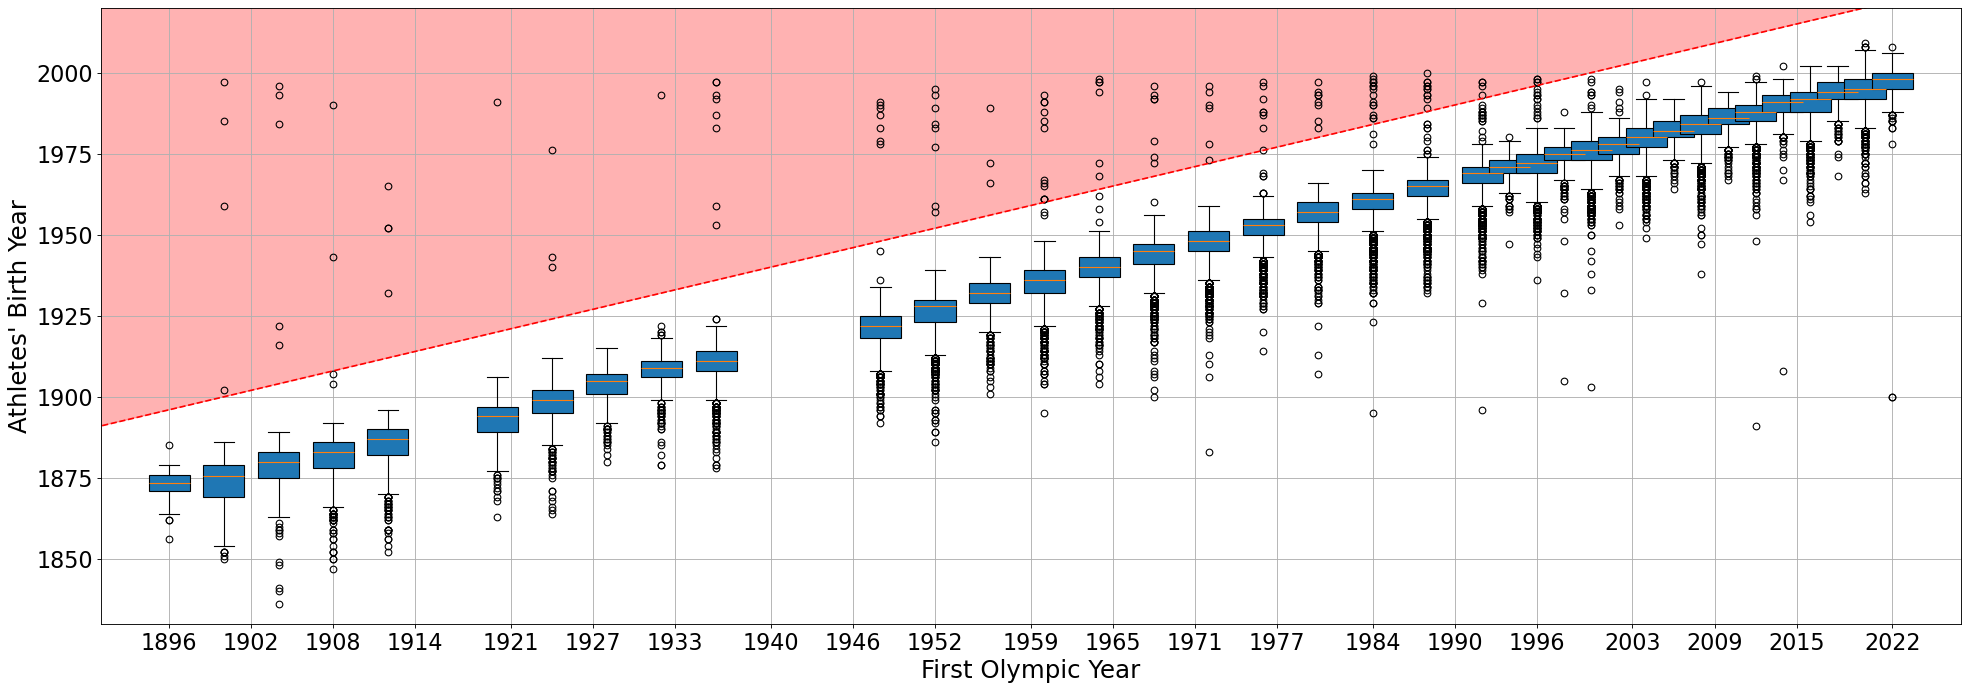
\includegraphics[width=\textwidth, keepaspectratio]{Distribution of Athletes' Birth Years by First Olympic Appearence.png}
    \caption{Distribution of Athletes' Birth Years by First Olympic Appearance}
    \label{fig:birth_years}
\end{figure}

\begin{figure}[ht]
    \centering
    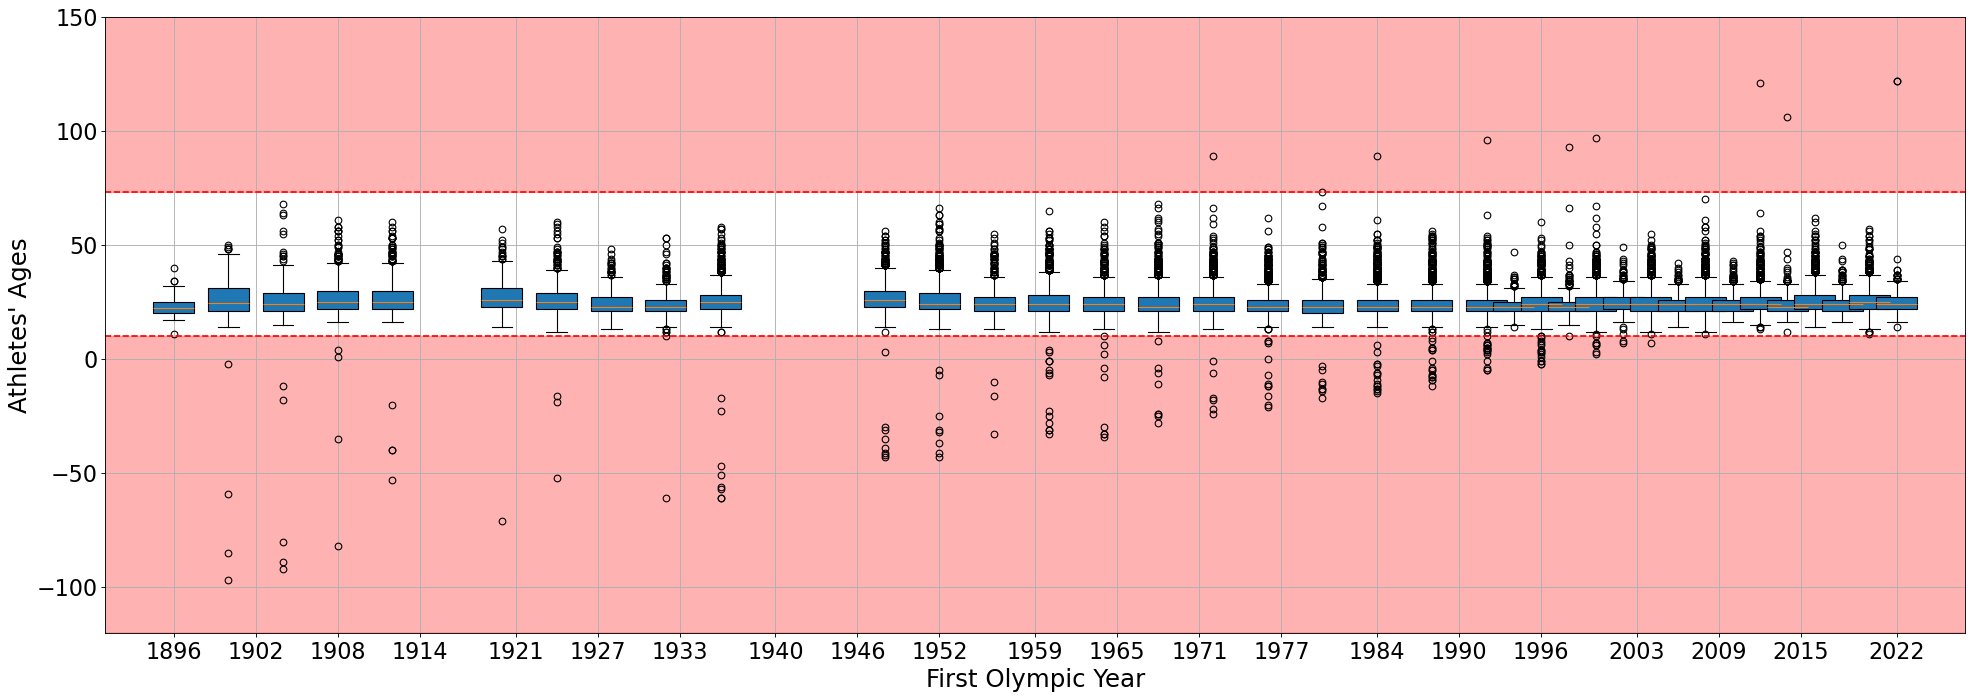
\includegraphics[width=\textwidth, keepaspectratio]{Distribution of Athletes' Ages at Their First Olympic Appearence.png}
    \caption{Distribution of Athletes' Ages at Their First Olympic Appearance}
    \label{fig:athlete_ages}
\end{figure}

\section{Ambiguous Geographical Data}

Geographical data in the raw dataset was often ambiguous or inconsistent. Key issues included:

\begin{itemize}
    \item \textbf{Host City and Country Mapping:} Host cities were inconsistently labeled or lacked corresponding country information. To resolve this, city names were mapped to their respective countries using geocoding tools such as Nominatim \cite{nominatim}.
    \item \textbf{Country Code Discrepancies:} Standardized two-letter (ISO 3166-1 alpha-2) and three-letter (ISO 3166-1 alpha-3) country codes were assigned to all entries to eliminate inconsistencies in naming conventions.
\end{itemize}

By standardizing geographical data, we ensured consistency and improved the dataset's usability for visualizations involving country-specific analyses.


\section{Missing Metadata}

A significant portion of the dataset contained missing or incomplete metadata, particularly for athletes and events. Common issues included:

\begin{itemize}
    \item \textbf{Incomplete Athlete Information:} Some athletes lacked URLs, full names, or demographic details. Such records were filtered out when critical information was unavailable.
    \item \textbf{Unresolved Medalist Metadata:} Certain medalists had incomplete associations with their events or disciplines, which limited their analytical use.
\end{itemize}

These gaps were addressed where possible, and records that could not be resolved were excluded from further analysis.


\chapter{Results} \label{chap:res}

\section{Analysis of Olympic Games Duration and Evolution}

The Gantt chart in Figure \ref{fig:gantt_olympics} illustrates the scheduling and duration of both Summer and Winter Olympic Games from the inaugural Athens Games in 1896 to the events in 2022. It highlights key milestones and trends in the evolution of the Olympics.

\begin{figure}[ht]
    \centering
    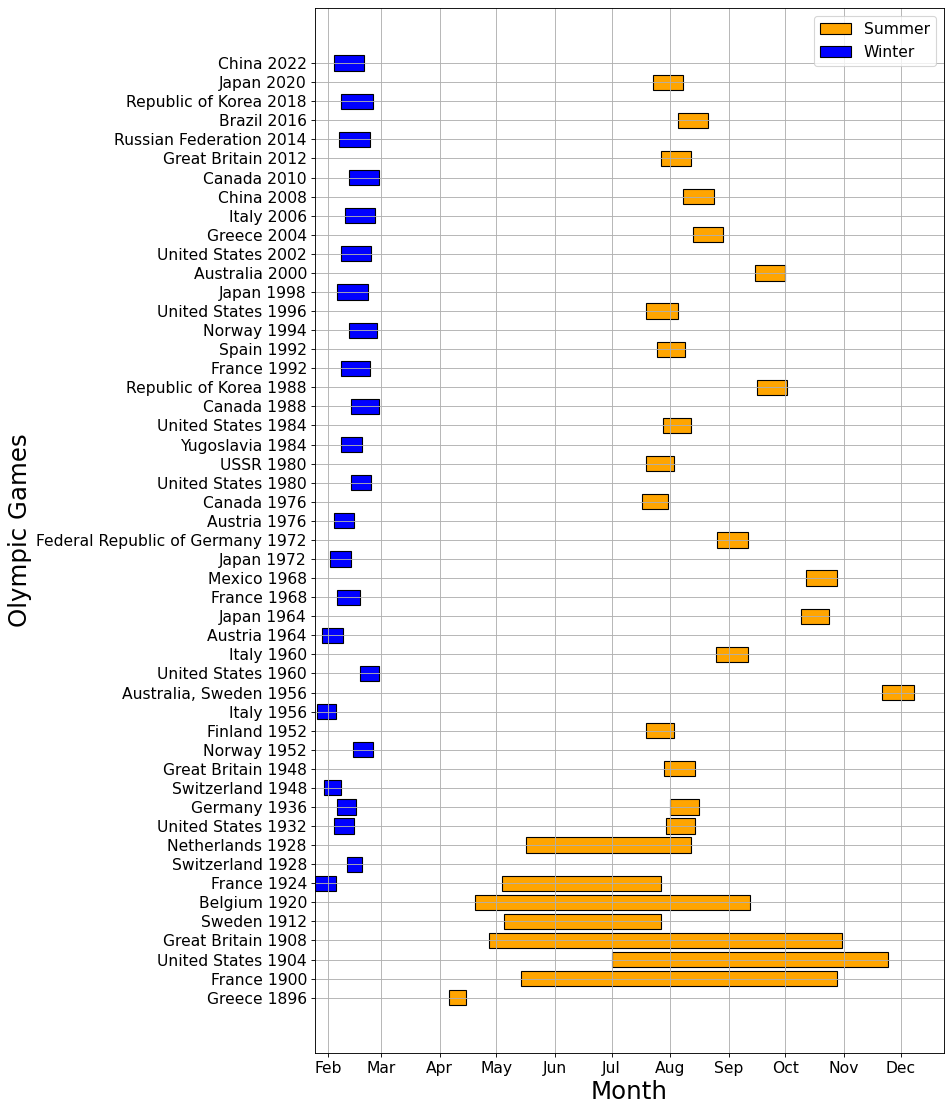
\includegraphics[width=0.8\textwidth]{Gantt Chart of Olympic Games.png}
    \caption{Gantt Chart of Olympic Games Duration}
    \label{fig:gantt_olympics}
\end{figure}

The modern Olympics began in 1896 with exclusively male participants and a limited schedule of events lasting 10 days. By 1900, the Paris Games introduced women's participation and expanded the schedule to over five months, integrating the Olympics into the World’s Fair. This unusual duration reflected the scattered organization and the addition of new sports like golf, tennis, and rowing. Over time, the duration became more standardized, with events typically lasting around two weeks by the mid-20th century, reflecting the Games' growing scale and complexity.

The Winter Olympics were introduced in Chamonix, France, in 1924, marking the start of a separate seasonal competition for winter sports. Notably, France hosted both the Summer and Winter Games in the same year, solidifying its pivotal role in Olympic history.

Additionally, the chart captures regular scheduling patterns, with Summer Games typically held between July and August and Winter Games in February. It also reveals disruptions caused by global conflicts, including cancellations during World War I and World War II.

\section{Chord Diagram for Migration Flow}

PLACEHOLDER ...

\section{Dynamic Choropleths and Bubble Maps}

The dynamic choropleth and bubble maps were designed to provide an interactive exploration of Olympic trends worldwide. These maps enable users to visualize data such as the frequency of Olympic hosting by country, the number of athlete debuts, and medal counts. With dynamic filtering options and multiple visualization styles, they offer a versatile and engaging way to analyze key aspects of Olympic history.

\begin{figure}[ht]
    \centering
    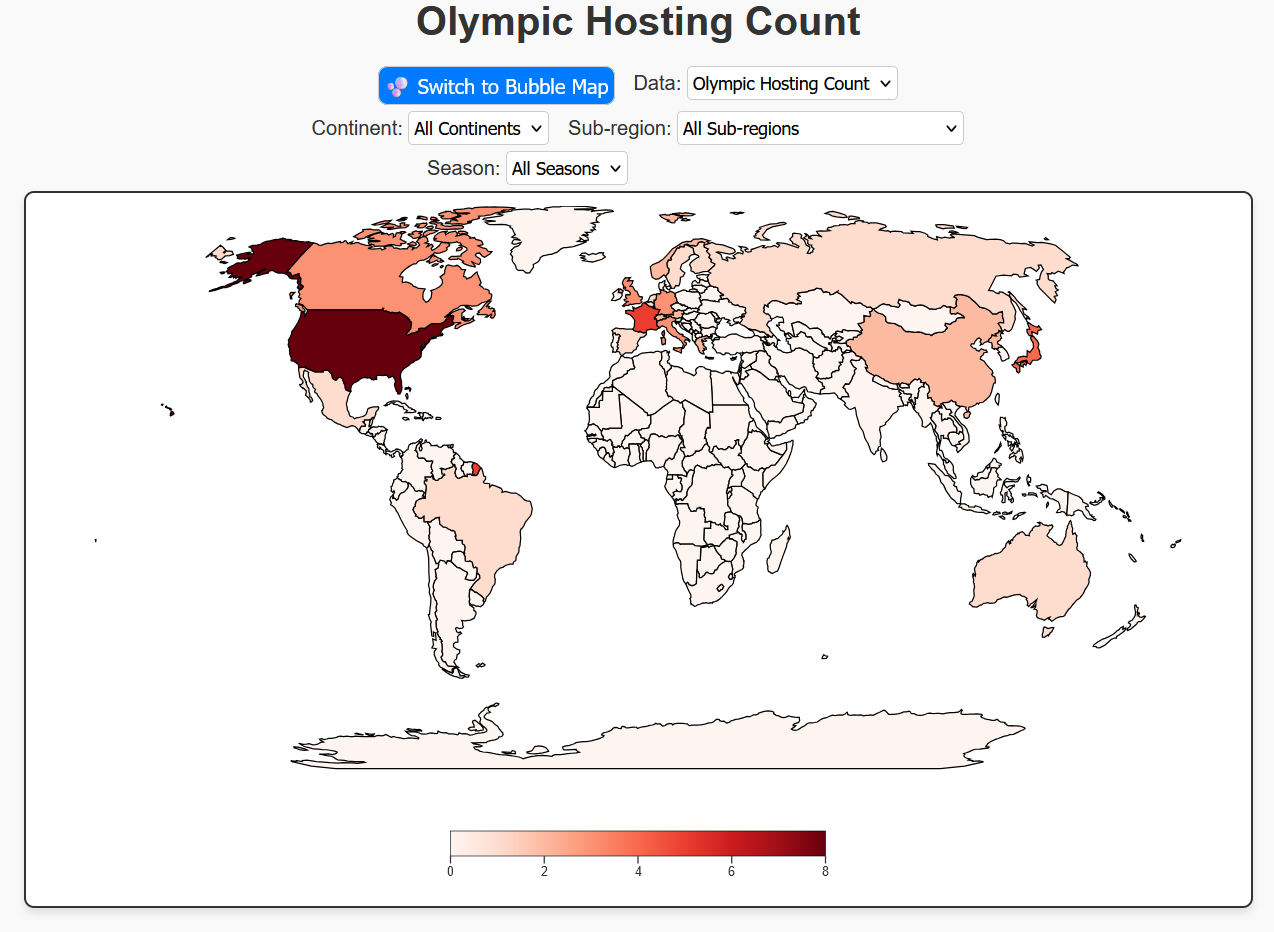
\includegraphics[width=0.8\textwidth]{Dynamic Choropleth.png}
    \caption{Dynamic Choropleth Map: Visualizing Olympic Hosting Trends}
    \label{fig:choropleth_map}
\end{figure}

\begin{figure}[ht]
    \centering
    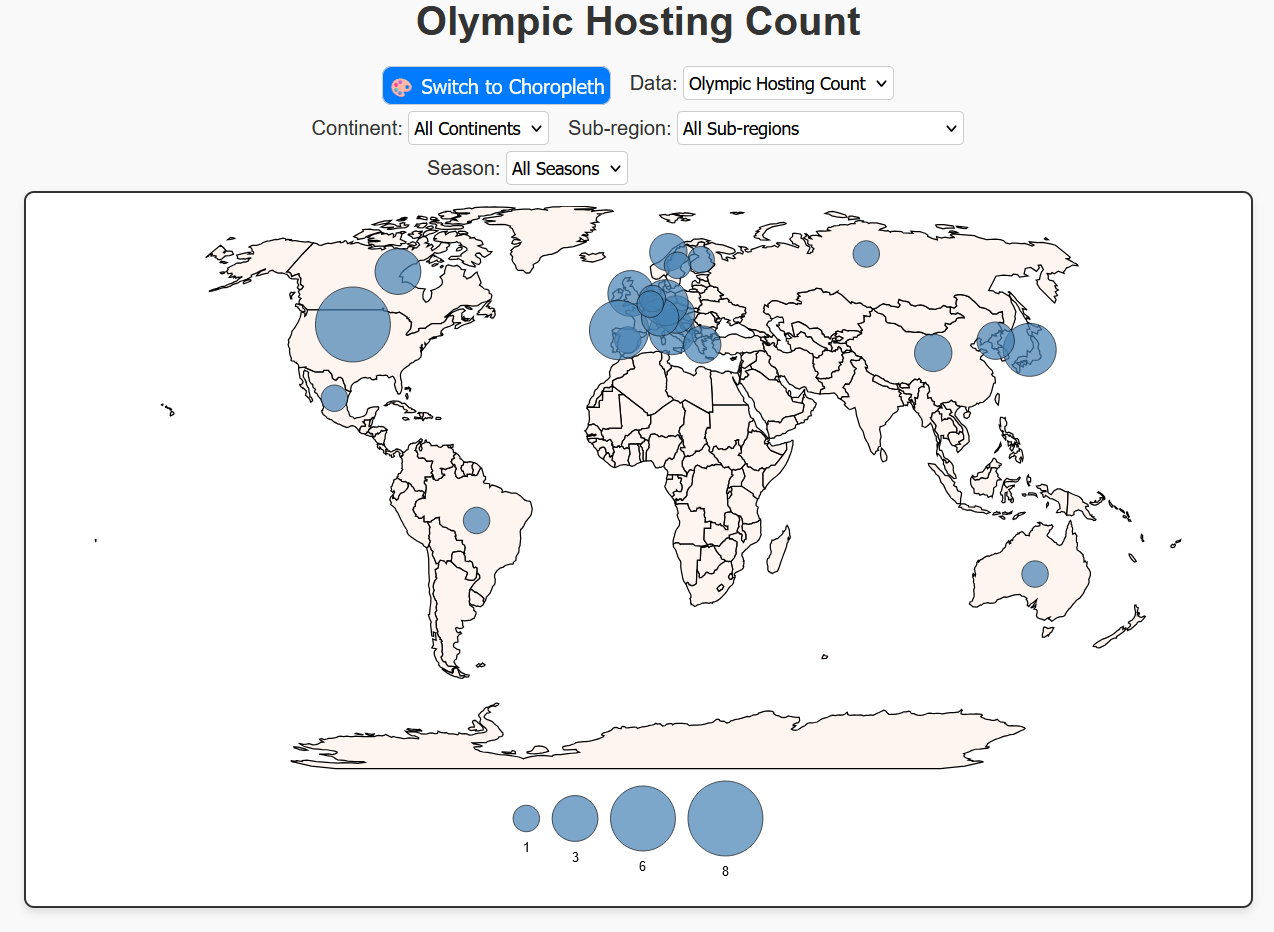
\includegraphics[width=0.8\textwidth]{Dynamic Bubble Map.png}
    \caption{Dynamic Bubble Map: Visualizing Olympic Hosting Trends}
    \label{fig:bubble_map}
\end{figure}

\subsection{Features of the Maps}

The maps provide the following functionalities:
\begin{itemize}
    \item \textbf{Visualization Modes:} Users can switch between a choropleth map (Figure \ref{fig:choropleth_map}) and a bubble map (Figure \ref{fig:bubble_map}) for different visual representations of hosting frequency.
    \item \textbf{Filters and Options:} Filtering options include continents, sub-regions, seasons (Summer or Winter), medal types (Gold, Silver or Bronze), if applicable. These allow users to customize the view and focus on specific geographic or temporal trends.
    \item \textbf{Interactivity:} Both maps feature hover-over tooltips displaying detailed information, such as the number of times a country has hosted the Olympics.
\end{itemize}

\subsection{Insights from the Maps}

These maps reveal several insights into Olympic hosting trends:
\begin{itemize}
    \item Countries such as the United States, Great Britain, and France stand out in number of debuts and high hosting frequencies, reflecting their longstanding involvement in the Olympics.
    \item Hosting occurrences are concentrated in Europe and North America, particularly during the early years of the modern Olympics.
    \item The inclusion of filtering options enables the identification of hosting trends by region, season, and medal type, highlighting the geographical expansion of the Games over time.
\end{itemize}

The combination of choropleth and bubble maps exemplifies the power of interactive visualizations, enabling a flexible exploration of the data while revealing key trends and disparities in Olympic hosting.

\section{ADNANE PLOTS}


\chapter{Conclusion and Future Work} \label{chap:conclusion}

In this work, we have created multiple plots to analyze Olympic Games data and uncover deeply embedded patterns within it. These visualizations have allowed us to derive new insights about the Olympics from both geographical and social perspectives.

In future work, Olympic Games data can be analyzed from political and economic perspectives. By integrating this data with economic indicators such as the GINI index(a measure of income inequality within a country) and GDP(Gross Domestic Product), it would be possible to gain deeper insights into how economic conditions and political factors influence participation, performance, and trends in the Olympics.


% Post-textual elements
\bibliography{doc/bibliography}
\appendix
\chapter{Complete dataset description} \label{app:A}

The \textit{Olympic Games Medals 1986-2022} dataset, sourced from Kaggle \cite{olympic_19862022}, contains comprehensive information about the Olympic Games spanning from 1986 to 2022. The data, originally scraped from the official International Olympic Committee website \cite{olympics}, includes details about athletes, medal results, hosting nations, and events. This section provides a complete overview of the dataset structure and its attributes.

The dataset consists of multiple files, each focusing on specific aspects of the Olympic Games. The key files and their contents are described below.

\section{olympic\_athletes.csv}

The file \texttt{olympic\_athletes.csv} includes the following attributes:

\begin{itemize}
    \item \texttt{athlete\_url}: The URL linking to the athlete's profile on the official Olympics website.
    \item \texttt{athlete\_full\_name}: The full name of the athlete.
    \item \texttt{games\_participations}: The total number of Olympic Games in which the athlete participated.
    \item \texttt{first\_game}: The first Olympic Games in which the athlete competed, specified by city and year.
    \item \texttt{athlete\_year\_birth}: The birth year of the athlete.
    \item \texttt{athlete\_medals}: The total medals won by the athlete across all participations.
    \item \texttt{bio}: A brief biographical summary or description of the athlete, if available, which is often not the case.
\end{itemize}

\section{olympic\_medals.csv}

The file \texttt{olympic\_medals.csv} includes the following attributes:

\begin{itemize}
    \item \texttt{discipline\_title}: The title of the sport or discipline (e.g., \texttt{Swimming}, \texttt{Athletics}).
    \item \texttt{slug\_game}: A unique identifier for the specific Olympic Games (e.g., \texttt{barcelona-1992}).
    \item \texttt{event\_title}: The title of the specific event within the discipline (e.g., \texttt{5000m men}, \texttt{parallel bars men}).
    \item \texttt{event\_gender}: The gender category of the event (\texttt{Men}, \texttt{Women}, or \texttt{Mixed} for mixed events).
    \item \texttt{medal\_type}: The type of medal awarded (\texttt{GOLD}, \texttt{SILVER}, or \texttt{BRONZE}).
    \item \texttt{participant\_type}: The type of participant (e.g., \texttt{Athlete} if individual, \texttt{GameTeam} otherwise).
    \item \texttt{participant\_title}: The name or title of the participant (e.g., team name or athlete name).
    \item \texttt{athlete\_url}: The URL linking to the athlete's profile (if applicable).
    \item \texttt{athlete\_full\_name}: The full name of the athlete (if applicable).
    \item \texttt{country\_name}: The name of the country associated with the medal-winning participant.
    \item \texttt{country\_code}: The two-letter country code (ISO 3166-1 alpha-2).
    \item \texttt{country\_3\_letter\_code}: The three-letter country code (ISO 3166-1 alpha-3).
\end{itemize}

\section{olympic\_hosts.csv}

The file \texttt{olympic\_hosts.csv} includes the following attributes:

\begin{itemize}
    \item \texttt{game\_slug}: A unique identifier for the specific Olympic Games (e.g., \texttt{barcelona-1992}).
    \item \texttt{game\_end\_date}: The end date of the Olympic Games.
    \item \texttt{game\_start\_date}: The start date of the Olympic Games.
    \item \texttt{game\_location}: The location of the Olympic Games (country).
    \item \texttt{game\_name}: The official name of the Olympic Games (e.g., \texttt{Oslo 1952}).
    \item \texttt{game\_season}: The season of the Games (\texttt{Summer} or \texttt{Winter}).
    \item \texttt{game\_year}: The year in which the Olympic Games took place.
\end{itemize}

\section{olympic\_results.csv}

The file \texttt{olympic\_results.csv} includes the following attributes:

\begin{itemize}
    \item \texttt{discipline\_title}: The title of the sport or discipline (e.g., \texttt{Swimming}, \texttt{Athletics}).
    \item \texttt{event\_title}: The title of the specific event within the discipline (e.g., \texttt{5000m men}, \texttt{tempest mixed}).
    \item \texttt{slug\_game}: A unique identifier for the specific Olympic Games (e.g., \texttt{montreal-1976}).
    \item \texttt{participant\_type}: The type of participant (e.g., \texttt{Athlete} if individual, \texttt{GameTeam} otherwise).
    \item \texttt{medal\_type}: The type of medal awarded (\texttt{GOLD}, \texttt{SILVER}, \texttt{BRONZE}, or \texttt{None} for participants who did not win a medal).
    \item \texttt{athletes}: A list of athletes associated with the participant (useful for team events).
    \item \texttt{rank\_equal}: Whether the rank is shared among multiple participants (\texttt{True} or \texttt{False}), if applicable.
    \item \texttt{rank\_position}: The rank of the participant in the event.
    \item \texttt{country\_name}: The name of the country associated with the participant.
    \item \texttt{country\_code}: The two-letter country code (ISO 3166-1 alpha-2).
    \item \texttt{country\_3\_letter\_code}: The three-letter country code (ISO 3166-1 alpha-3).
    \item \texttt{athlete\_url}: The URL linking to the athlete's profile (if applicable).
    \item \texttt{athlete\_full\_name}: The full name of the athlete (if applicable).
    \item \texttt{value\_unit}: The unit of measurement for performance values (e.g., seconds, meters).
    \item \texttt{value\_type}: The type of performance value recorded (e.g., time, distance).
\end{itemize}

\section{Dataset Summary}

The dataset provides detailed information about:
\begin{itemize}
    \item Over 120 years of Olympic Games history, spanning Summer and Winter Games.
    \item Thousands of athletes from different countries, disciplines, and events.
    \item Medal counts and distribution patterns across various sports and seasons.
    \item Host cities and countries, offering geographical insights into the Games.
\end{itemize}


\annex
\chapter{Numerical data of simulations} \label{an:A}

Example of long tables that cross pages.

\setstretch{1.3}

\begin{center}
\begin{longtable}{*{5}{c}}
	\caption{System's output for all scenarios.}\\
	\specialrule{1.5pt}{2pt}{2pt}
	Time	& Scenario 1	& Scenario 2	& Scenario 3	& Scenario 4 \\
	\specialrule{0.1pt}{2pt}{2pt}
	\endfirsthead

	\specialrule{1.5pt}{2pt}{2pt}
	Time	& Scenario 1	& Scenario 2	& Scenario 3	& Scenario 4 \\
	\specialrule{0.1pt}{2pt}{2pt}
	\endhead

	\specialrule{0.3pt}{2pt}{2pt}
	\multicolumn{5}{c}{{Continued on next page}} \\
	\specialrule{0.3pt}{2pt}{2pt}
	\endfoot
	\endlastfoot

		1	& 1.3	& 1.2	& 1.1	& 1.0\\
		2	& 2.4	& 1.9	& 1.6	& 1.0\\
		3	& 3.7	& 2.8	& 2.1	& 1.1\\
		4	& 5.2	& 3.7	& 2.7	& 1.2\\
		5	& 6.7	& 4.7	& 3.4	& 1.2\\
		6	& 8.2	& 5.7	& 4.0	& 1.3\\
		7	& 9.7	& 6.7	& 4.6	& 1.3\\
		8	& 11.1	& 7.6	& 5.2	& 1.4\\
		9	& 12.4	& 8.4	& 5.7	& 1.4\\
		10	& 13.6	& 9.2	& 6.2	& 1.4\\
		11	& 14.7	& 9.9	& 6.7	& 1.5\\
		12	& 15.7	& 10.6	& 7.1	& 1.5\\
		13	& 16.7	& 11.2	& 7.5	& 1.5\\
		14	& 17.5	& 11.7	& 7.8	& 1.5\\
		15	& 18.3	& 12.2	& 8.1	& 1.6\\
		16	& 18.9	& 12.7	& 8.4	& 1.6\\
		17	& 19.5	& 13.1	& 8.6	& 1.6\\
		18	& 20.0	& 13.4	& 8.9	& 1.6\\
		19	& 20.5	& 13.7	& 9.0	& 1.6\\
		20	& 20.9	& 13.9	& 9.2	& 1.6\\
		\specialrule{0.3pt}{2pt}{2pt}
		\multicolumn{5}{c}{Source: Author.}
\end{longtable}

%
\begin{longtable}{*{5}{c}}
	\caption{System's output variance for all scenarios.}\\
	\specialrule{1.5pt}{2pt}{2pt}
	Time	& Scenario 1	& Scenario 2	& Scenario 3	& Scenario 4 \\
	\specialrule{0.1pt}{2pt}{2pt}
	\endfirsthead

	\specialrule{1.5pt}{2pt}{2pt}
	Time	& Scenario 1	& Scenario 2	& Scenario 3	& Scenario 4 \\
	\specialrule{0.1pt}{2pt}{2pt}
	\endhead

	\specialrule{0.3pt}{2pt}{2pt}
	\multicolumn{5}{c}{{Continued on next page}} \\
	\specialrule{0.3pt}{2pt}{2pt}
	\endfoot
	\endlastfoot
		1	& 0.86	& 0.37	& 0.15	& 0.0007\\
		2	& 3.54	& 1.50	& 0.60	& 0.003\\
		3	& 6.19	& 2.62	& 1.05	& 0.005\\
		4	& 8.25	& 3.49	& 1.40	& 0.007\\
		5	& 9.58	& 4.05	& 1.62	& 0.008\\
		6	& 10.21	& 4.32	& 1.73	& 0.009\\
		7	& 10.30	& 4.36	& 1.74	& 0.009\\
		8	& 9.97	& 4.22	& 1.69	& 0.008\\
		9	& 9.37	& 3.96	& 1.58	& 0.008\\
		10	& 8.58	& 3.63	& 1.45	& 0.007\\
		11	& 7.70	& 3.25	& 1.30	& 0.007\\
		12	& 6.78	& 2.87	& 1.15	& 0.006\\
		13	& 5.87	& 2.48	& 0.99	& 0.005\\
		14	& 5.01	& 2.12	& 0.85	& 0.004\\
		15	& 4.20	& 1.78	& 0.71	& 0.004\\
		16	& 3.48	& 1.47	& 0.59	& 0.003\\
		17	& 2.84	& 1.20	& 0.48	& 0.002\\
		18	& 2.28	& 0.97	& 0.39	& 0.002\\
		19	& 1.81	& 0.77	& 0.31	& 0.002\\
		20	& 1.42	& 0.60	& 0.24	& 0.001\\
		\specialrule{0.3pt}{2pt}{2pt}
		\multicolumn{5}{c}{Source: Author.}
\end{longtable}

%
\begin{longtable}{*{6}{c}}
	\caption{Control policy for scenario A.}\\
	\specialrule{1.5pt}{2pt}{2pt}
	Time	& CDI	& EMBR3	& ITUB4	& PETR4	& VALE5 \\
	\specialrule{0.1pt}{2pt}{2pt}
	\endfirsthead

	\specialrule{1.5pt}{2pt}{2pt}
	Time	& CDI	& EMBR3	& ITUB4	& PETR4	& VALE5 \\
	\specialrule{0.1pt}{2pt}{2pt}
	\endhead

	\specialrule{0.3pt}{2pt}{2pt}
	\multicolumn{6}{c}{{Continued on next page}} \\
	\specialrule{0.3pt}{2pt}{2pt}
	\endfoot
	\endlastfoot

		0	& -137.9	& -24.9	& 87.1	& 9.8	& 66.9\\
		1	& -138.7	& -21.8	& 88.5	& 15.5	& 57.8\\
		2	& -136.0	& -20.0	& 87.3	& 17.4	& 53.6\\
		3	& -126.9	& -18.2	& 82.3	& 17.4	& 49.1\\
		4	& -116.2	& -16.5	& 76.4	& 17.0	& 44.5\\
		5	& -109.6	& -15.5	& 72.9	& 16.3	& 42.6\\
		6	& -100.9	& -14.3	& 68.3	& 15.6	& 39.6\\
		7	& -94.8		& -13.3	& 65.1	& 14.8	& 37.8\\
		8	& -87.0		& -12.0	& 60.9	& 14.2	& 35.0\\
		9	& -73.2		& -11.0	& 53.5	& 12.5	& 30.6\\
		10	& -65.9		& -10.0	& 49.4	& 11.5	& 28.5\\
		11	& -51.4		& -9.2	& 41.5	& 9.6	& 24.2\\
		12	& -43.2		& -8.4	& 37.0	& 8.3	& 22.0\\
		13	& -37.8		& -7.2	& 34.1	& 7.9	& 19.7\\
		14	& -29.9		& -6.4	& 29.7	& 6.9	& 17.2\\
		15	& -23.2		& -5.4	& 25.9	& 6.1	& 14.8\\
		16	& -16.6		& -4.6	& 22.2	& 5.2	& 12.8\\
		17	& -12.7		& -3.9	& 20.0	& 4.7	& 11.4\\
		18	& -7.0		& -3.3	& 16.8	& 3.9	& 9.7\\
		19	& -1.6		& -2.7	& 13.7	& 3.3	& 7.7\\
		\specialrule{0.3pt}{2pt}{2pt}
		\multicolumn{6}{c}{Source: Author.}
\end{longtable}

%
\begin{longtable}{*{6}{c}}
	\caption{Control policy for scenario B.}\\
	\specialrule{1.5pt}{2pt}{2pt}
	Time	& CDI	& EMBR3	& ITUB4	& PETR4	& VALE5 \\
	\specialrule{0.1pt}{2pt}{2pt}
	\endfirsthead

	\specialrule{1.5pt}{2pt}{2pt}
	Time	& CDI	& EMBR3	& ITUB4	& PETR4	& VALE5 \\
	\specialrule{0.1pt}{2pt}{2pt}
	\endhead

	\specialrule{0.3pt}{2pt}{2pt}
	\multicolumn{6}{c}{{Continued on next page}} \\
	\specialrule{0.3pt}{2pt}{2pt}
	\endfoot
	\endlastfoot

		0	& -89.3		& -16.2	& 56.6	& 6.4	& 43.5\\
		1	& -89.3		& -14.0	& 57.2	& 10.2	& 37.1\\
		2	& -85.8		& -12.9	& 55.4	& 11.0	& 34.2\\
		3	& -80.5		& -11.8	& 52.6	& 11.1	& 31.5\\
		4	& -76.7		& -11.1	& 50.5	& 11.0	& 30.0\\
		5	& -74.3		& -10.3	& 49.4	& 11.0	& 28.9\\
		6	& -63.1		& -9.4	& 43.2	& 9.7	& 25.4\\
		7	& -57.4		& -8.6	& 40.2	& 9.2	& 23.3\\
		8	& -50.3		& -7.9	& 36.3	& 8.4	& 21.1\\
		9	& -45.8		& -7.2	& 33.9	& 7.9	& 19.5\\
		10	& -38.0		& -6.6	& 29.6	& 6.7	& 17.4\\
		11	& -35.3		& -5.8	& 28.2	& 6.6	& 16.3\\
		12	& -29.3		& -5.3	& 25.0	& 5.8	& 14.4\\
		13	& -24.1		& -4.6	& 22.0	& 5.2	& 12.7\\
		14	& -19.0		& -4.2	& 19.2	& 4.3	& 11.4\\
		15	& -14.9		& -3.6	& 17.0	& 3.9	& 9.9\\
		16	& -10.5		& -3.1	& 14.4	& 3.3	& 8.5\\
		17	& -7.1		& -2.6	& 12.6	& 3.0	& 7.2\\
		18	& -4.4		& -2.1	& 11.0	& 2.6	& 6.2\\
		19	& -0.3		& -1.7	& 8.7	& 2.1	& 4.9\\
		\specialrule{0.3pt}{2pt}{2pt}
		\multicolumn{6}{c}{Source: Author.}
\end{longtable}

\end{center}

\vfill
\setstretch{\doubleSpacingRate}


\end{document}
